\documentclass{beamer}

\usepackage[english]{babel}
\usepackage{minted}
\newcommand{\mil}[1]{\mintinline{java}{#1}}
\usepackage{upquote}
\usepackage{graphicx}
\usepackage{tikz}
\usepackage{hyperref}
\usetikzlibrary{matrix,backgrounds}
\usepackage{hyperref}

\title[]{JavaFX}
\subtitle{Basic Procedure for Building JavaFX Apps} % (optional)

\author[]{Dalton State College} 

%\institute[Dalton State College]

\date[T. Gonzalez]{T. Gonzalez}

% If you wish to uncover everything in a step-wise fashion, uncomment
% the following command: 

%\beamerdefaultoverlayspecification{<+->}

\begin{document}

\begin{frame}

	\titlepage
	
\end{frame}

\begin{frame}
    
        1.  Open up eclipse and choose File > New > Other
        
        \begin{center}
            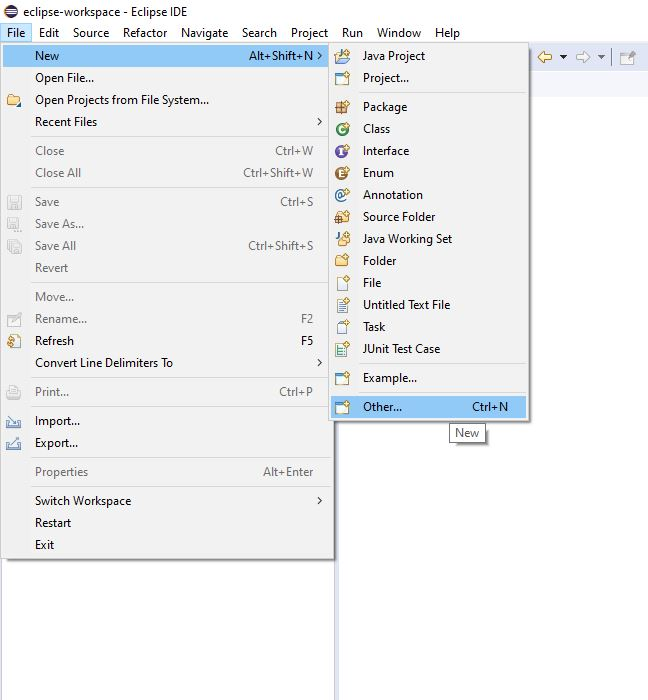
\includegraphics[scale=.4]{file_new_other.jpg}
        \end{center}
        
\end{frame}

\begin{frame}

        2.  Choose JavaFX > JavaFXProject and then click Next

        \begin{center}
            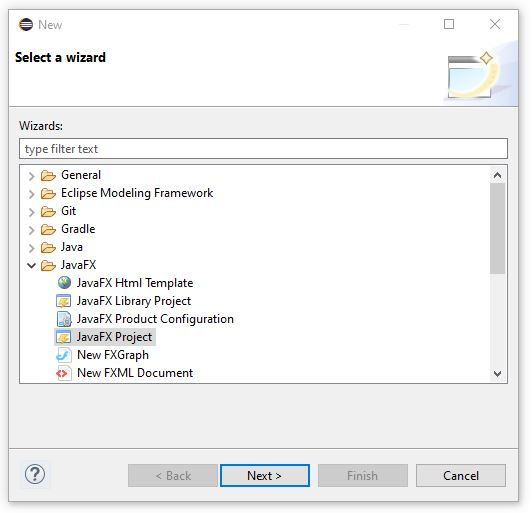
\includegraphics[scale=.4]{java_fx_project.jpg}
        \end{center}
        
\end{frame}

\begin{frame}

        3.  Type project name and click Next.  Adjust default location if desired and then click Next.

        \begin{center}
            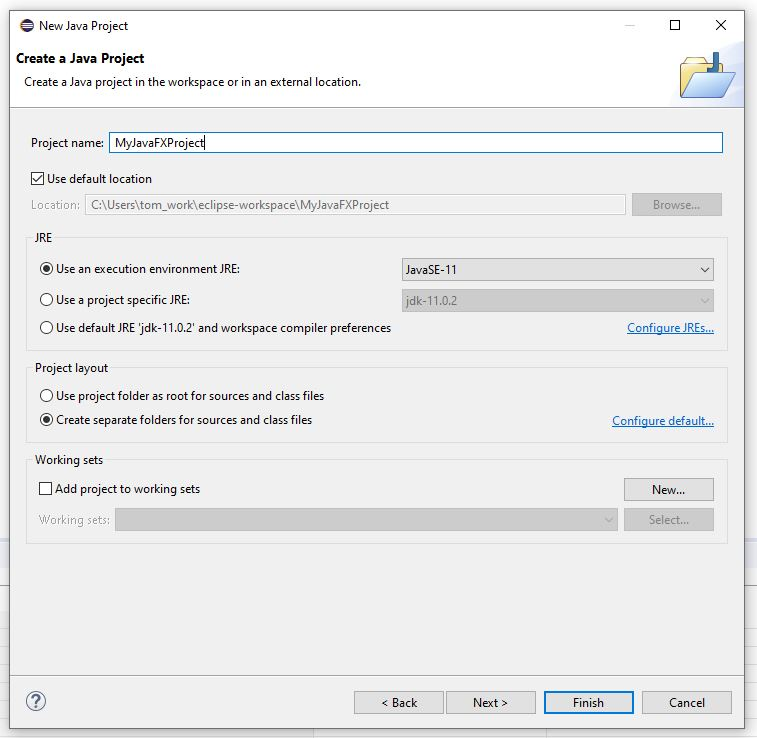
\includegraphics[scale=.35]{my_java_fx_project.jpg}
        \end{center}
        
\end{frame}

\begin{frame}
        
        4.  Uncheck create module-info.java (optional) and then click Next.

        \begin{center}
            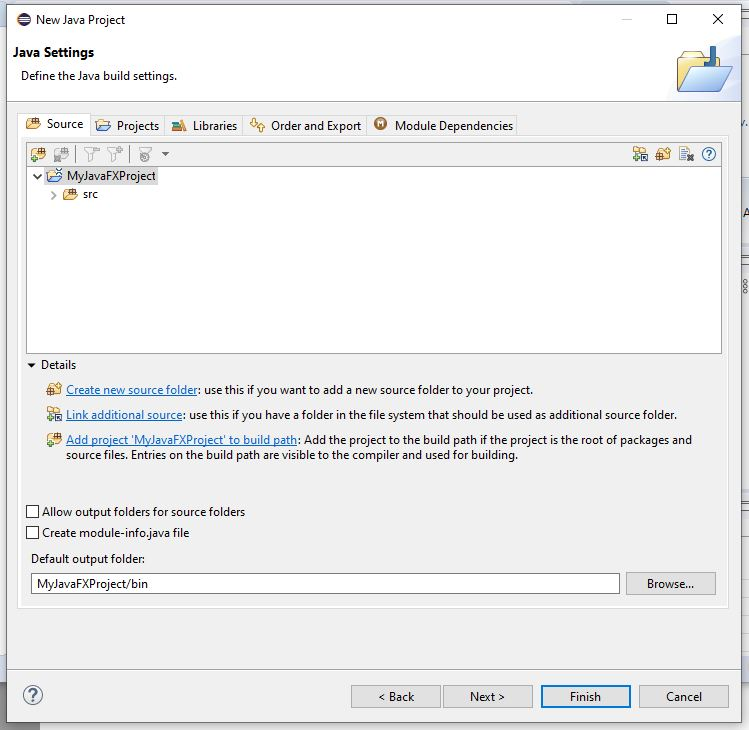
\includegraphics[scale=.35]{java_settings.jpg}
        \end{center}
\end{frame}
\begin{frame}
    \begin{enumerate}
        \item[5.]  Choose FXML for language.       
        \item[6.]  Choose a container for root-type.
        \item[7.]  Choose a file name.
        \item[8.]  Choose a Controller name.
        \item[9.]  Click Finish.
    \end{enumerate}  
    
        \begin{center}
            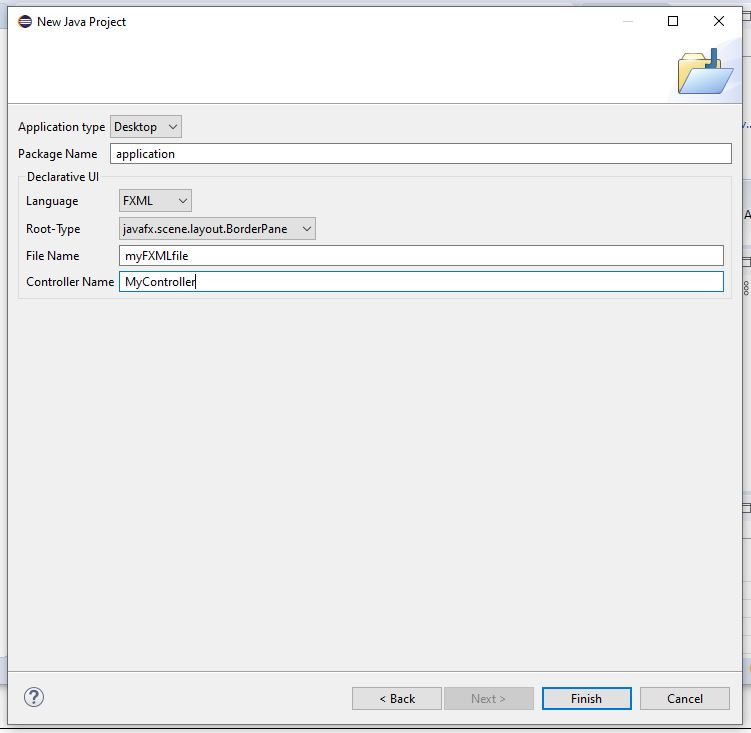
\includegraphics[scale=.3]{settings.jpg}
        \end{center}      
\end{frame}

\begin{frame}        
        10.  Find your FXML file in the Package Explorer, right click and choose Open with Scene Builder.

        \begin{center}
            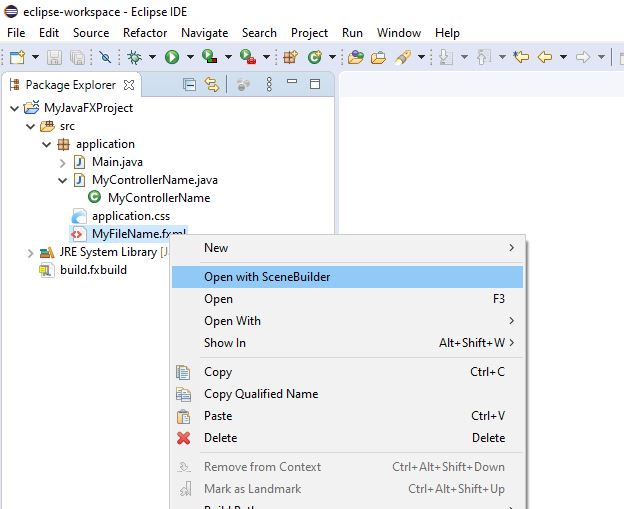
\includegraphics[scale=.35]{open_with_scene_builder.jpg}
        \end{center}
     
\end{frame}

\begin{frame}        
        11.  In Scene Builder, you might have to resize your root container to make it visible.
        
        \begin{itemize}
            \item Click on your root container in the Hierarchy tab.
            \item Under Layout click on Pref Width and set to 600, then click on Pref Height and set to 400. 
        \end{itemize}
        

        \begin{center}
            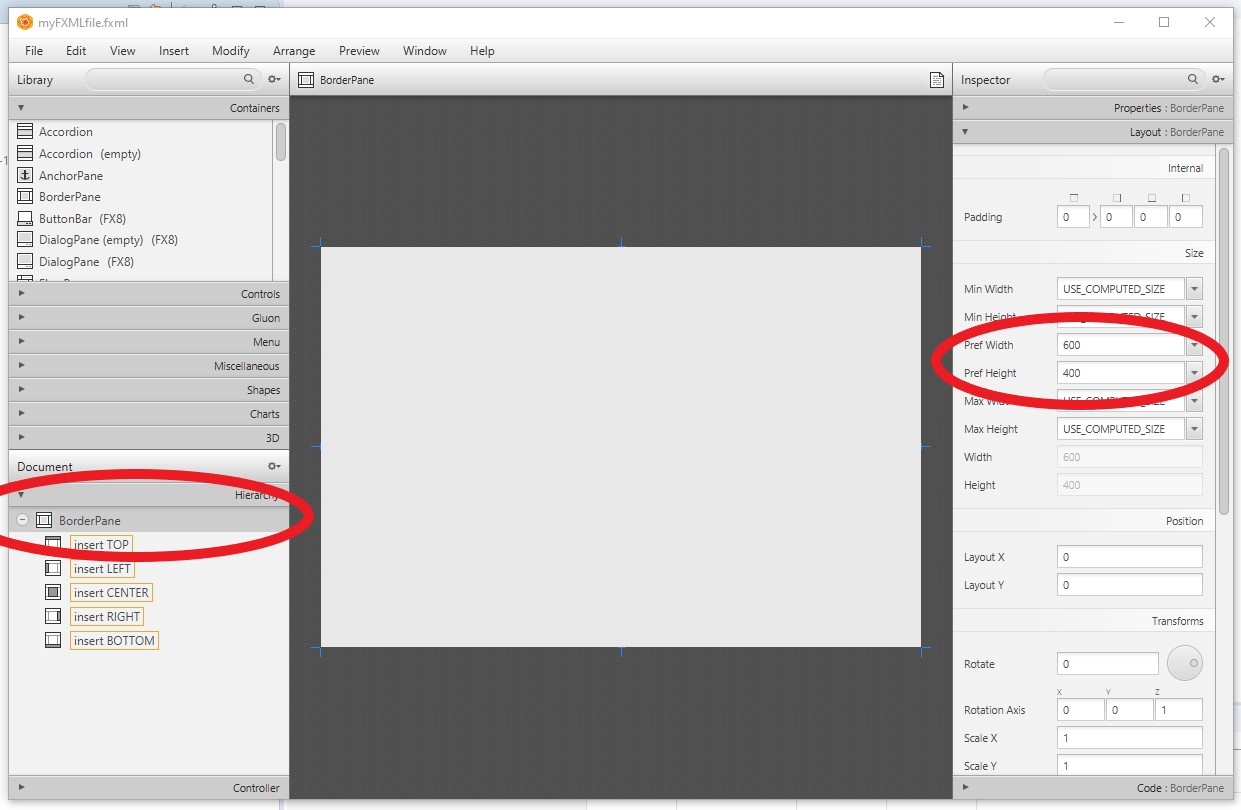
\includegraphics[scale=.2]{resize.jpg}
        \end{center}
           
\end{frame}

\begin{frame}
12. Drag other controls and containers from the Library Panel to
the Content Panel.

        \begin{center}
            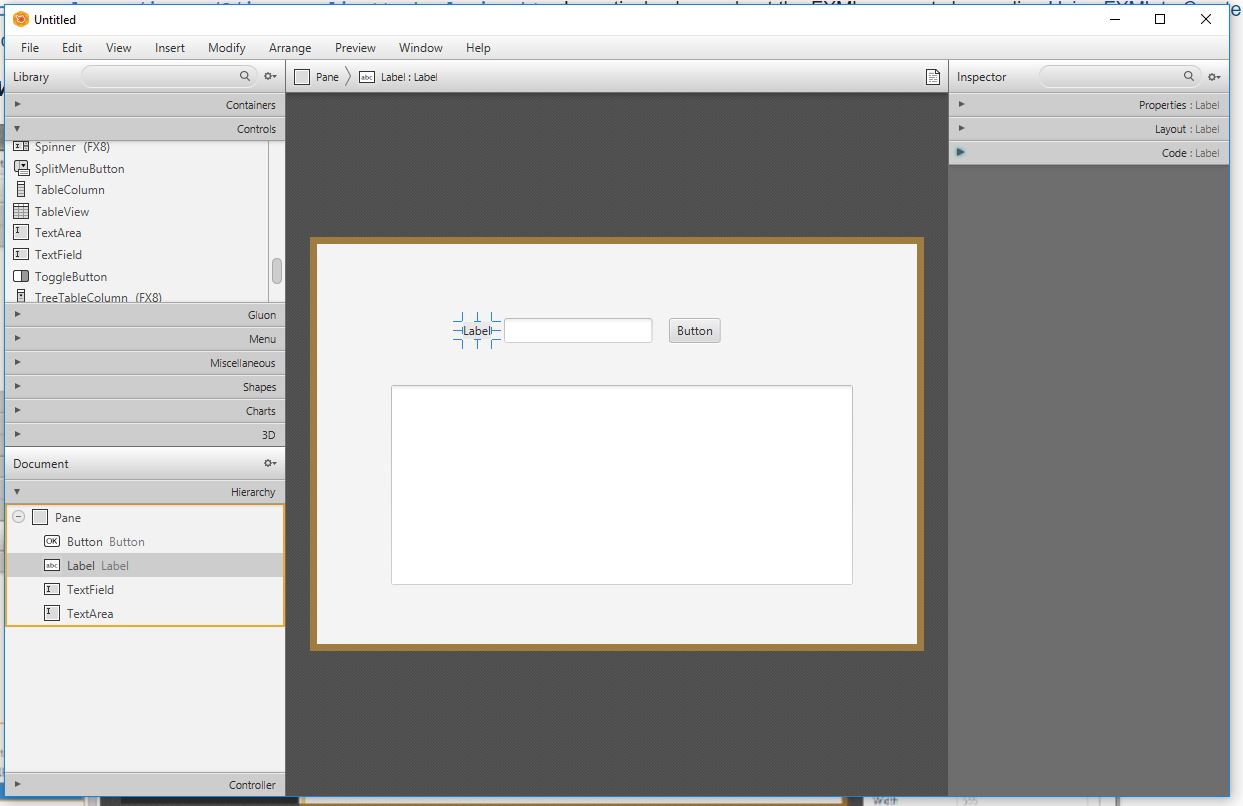
\includegraphics[scale=.3]{step2.jpg}
        \end{center}
        
\end{frame}

\begin{frame}
13. Adjust a control’s properties by clicking on the control,
choosing Properties from the Inspector Panel, and changing the
desired property.

        \begin{center}
            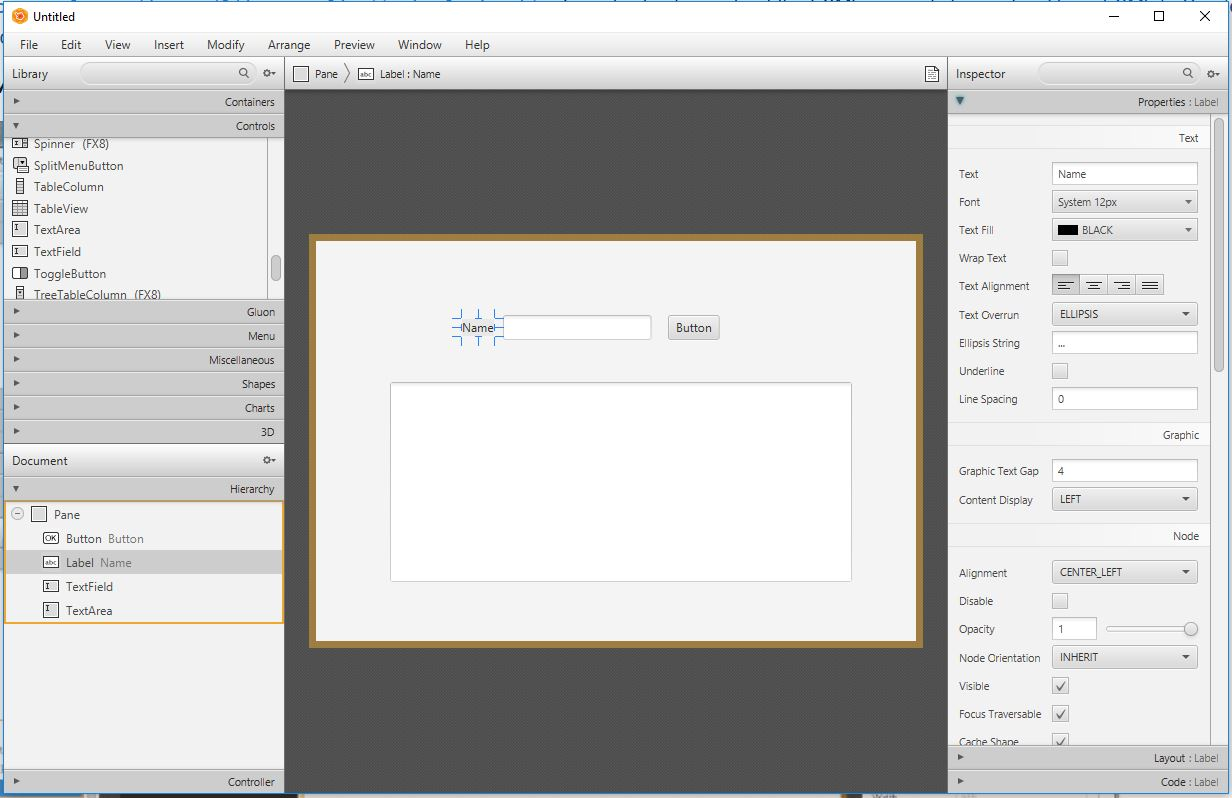
\includegraphics[scale=.3]{step3.jpg}
        \end{center}
\end{frame}

\begin{frame}
14. Adjust each control’s fxid and event handler (if applicable) by clicking on the control, choosing Code from the Inspector Panel, and changing the value for fxid and On Action text field.

        \begin{center}
            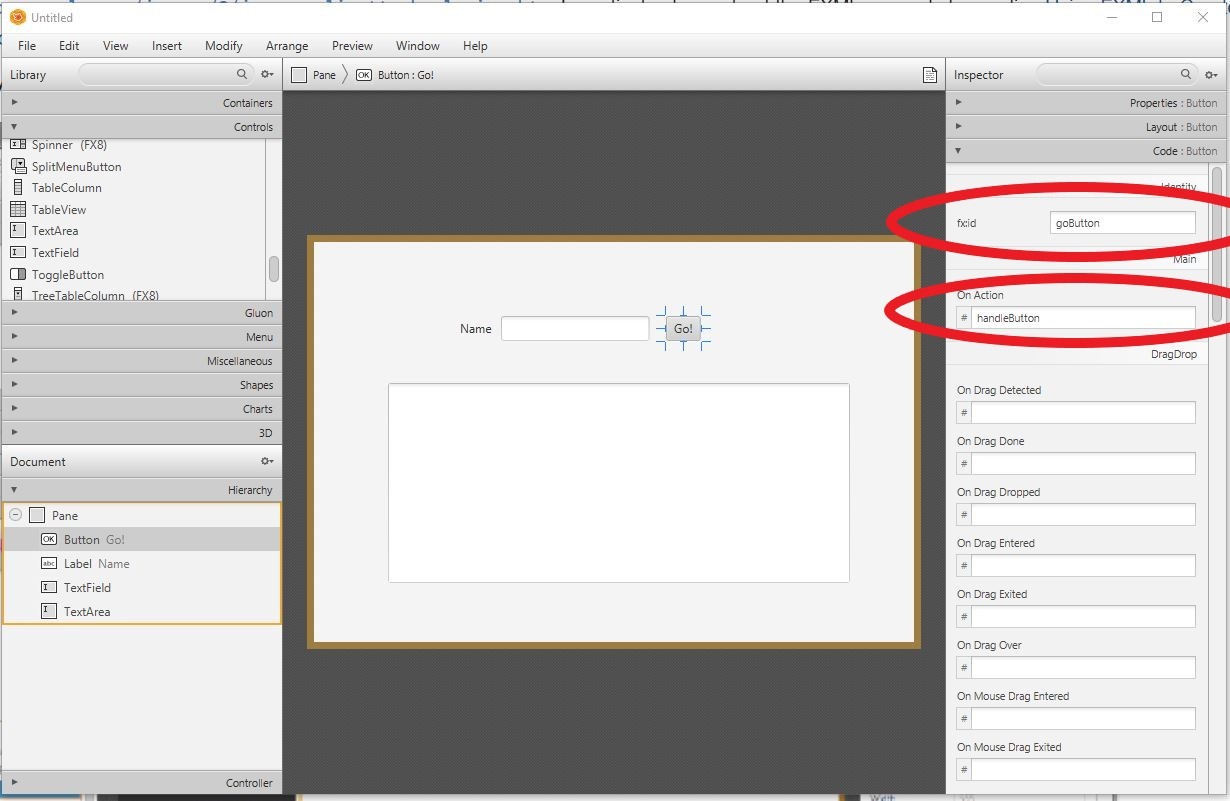
\includegraphics[scale=.3]{step4.jpg}
        \end{center}
\end{frame}

\begin{frame}
15. Save the file, close Scene Builder, and go back to eclipse.
\end{frame}

\begin{frame}
16. In eclipse, right click and delete the existing controller.
        \begin{center}
            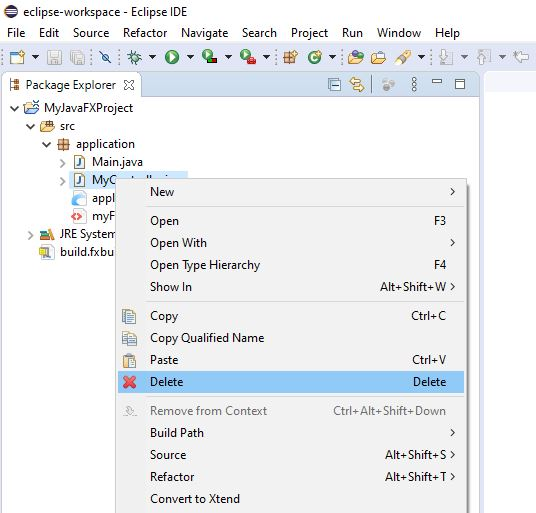
\includegraphics[scale=.4]{delete_controller.jpg}
        \end{center}
\end{frame}

\begin{frame}
17. Open the FXML file by double clicking on it.
        \begin{center}
            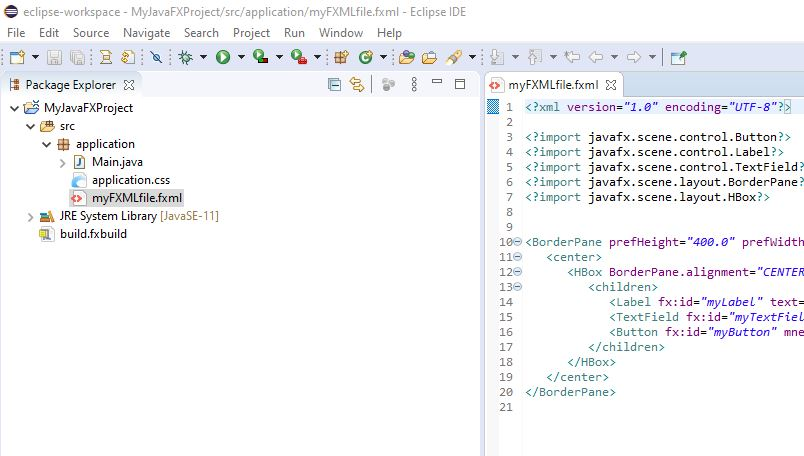
\includegraphics[scale=.4]{open_fxml.jpg}
        \end{center}

\end{frame}

\begin{frame}
18. Right-click within the FXML document and choose Source > Generate Controller, and then click OK.

        \begin{center}
            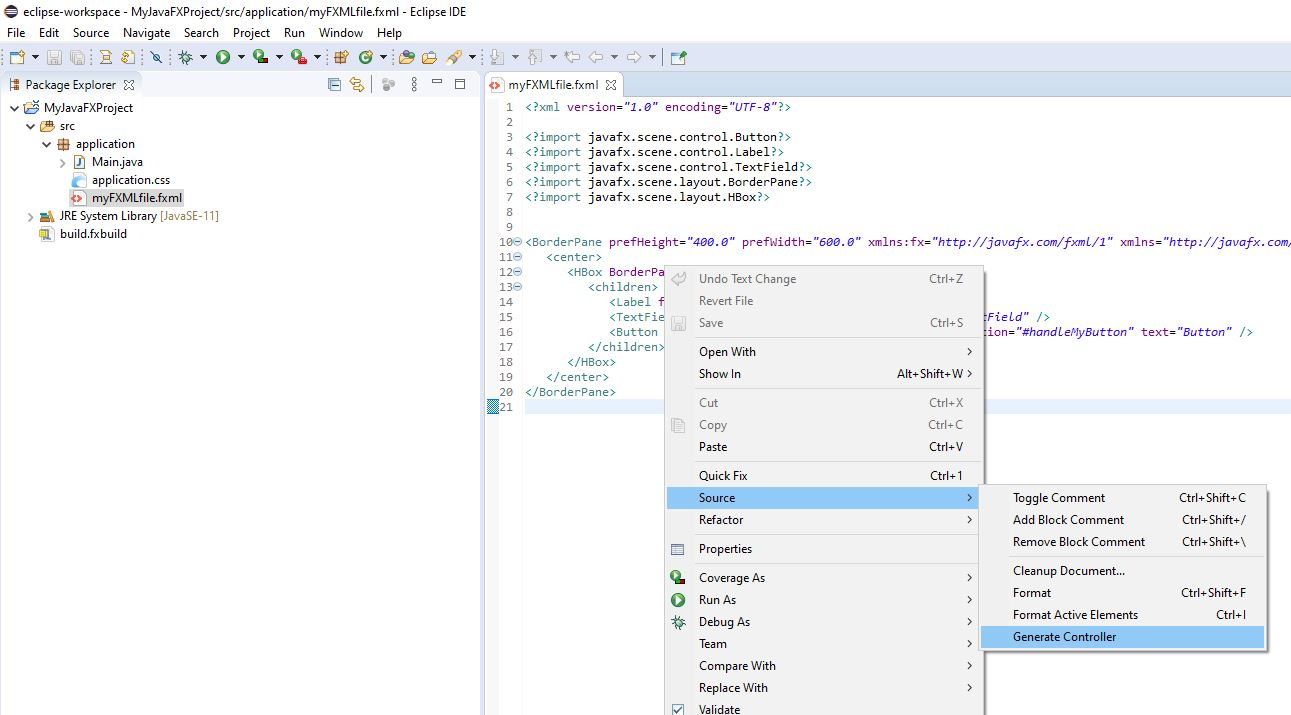
\includegraphics[scale=.2]{generate_controller.jpg}
        \end{center}
\end{frame}

\begin{frame}
19. Open the controller file and add your event handling code to the Event Listener methods.
        \begin{center}
            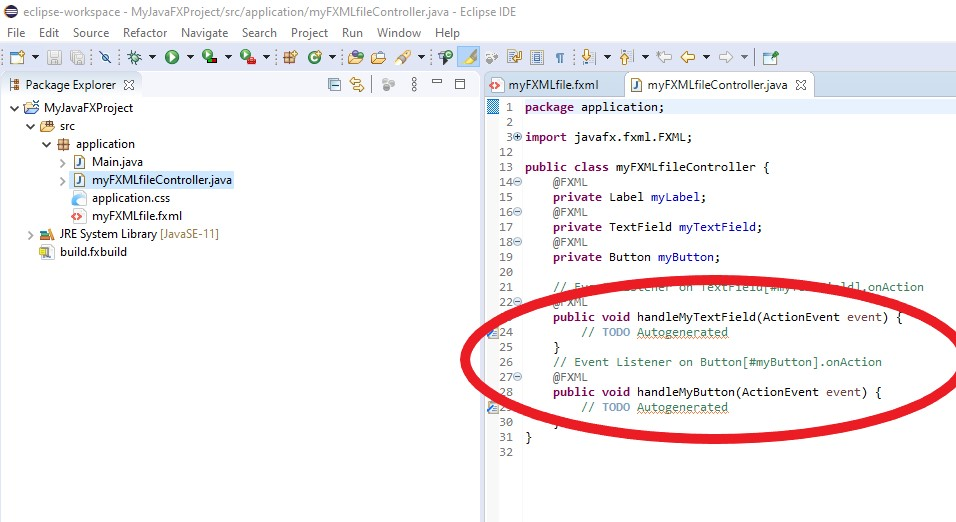
\includegraphics[scale=.2]{event_listeners.jpg}
        \end{center}
\end{frame}

\begin{frame}{In-Class Problem}

Write a JavaFX program with a Label, TextField, Button, and TextArea.  When the user types their name into the TextField and then clicks the Button, the message Hello <Name> is displayed where <Name> is the text that the user entered in the TextField.
\end{frame}

\begin{frame}

    \frametitle{In-Class Problem}
    
Write a JavaFX program with two buttons and a \mil{Text} object.  Clicking on one button should move the \mil{Text} object to the left and clicking on the other button should move the \mil{Text} object to the right.
  
\end{frame}

\begin{frame}

    \frametitle{In-Class Problem}
    
Write a JavaFX program that converts miles to kilometers and vice versa.  The GUI should have two \mil{TextField}s, one for miles and one for kilometers.  If you enter a value in the miles \mil{TextField} and press the enter key, the corresponding kilometer value is displayed in the kilometers \mil{TextField}.  Likewise, if you enter a value in the kilometer \mil{TextField} and press the Enter key, the corresponding mile value is displayed in the mile \mil{TextField}.    
\end{frame}

\begin{frame}

    \frametitle{In-Class Problem}
    
 Write a JavaFX program that lets the user enter a loan amount and loan period in number of years and displays the monthly and total payments for each interest rate starting from 5\% to 8\%, with an increment of 1/8.  The user interface should include two \mil{TextField}s, one for the loan amount, one for the number of years.  The user interface should also contain a \mil{Button}.  When the user clicks the button, the results should be displayed in a \mil{TextArea}.  The next slide shows a sample run.
\end{frame}

\begin{frame}[fragile]
\begin{verbatim}
Loan Amount:  10000
Number of Years:  5

Interest Rate      Monthly Payment     Total Payment
 5.000%             $188.71             $11,322.74
 5.125%             $189.28             $11,357.13
 5.250%             $189.85             $11,391.59
 ...
 7.875%             $202.17             $12,129.97
 8.000%             $202.76             $12,165.83 
\end{verbatim}
\end{frame}

\end{document}